% QUESTAO
O valor do \^angulo $x$ na figura \'e:

\parbox{0.27\linewidth}{

% ALTERNATIVAS
$105º$
$90º$
$120º$
$135º$
$110º$

}\parbox{0.72\linewidth}{
\begin{center}
\vspace{-3mm}
\begin{tikzpicture}[scale=0.95]
\def\legA{}
\def\legB{}
\def\legC{$x$}
\triangulo
{$12\sqrt{2}$}	              {12*sqrt(2)}	               {45}
{$12$}		  {12}	               {0}
{}	              {0}	               {0}
\end{tikzpicture}
\vspace{-9mm}
\end{center}
}


